\documentclass[../main.tex]{subfiles}

\begin{document}

\part{Roots and Optimization}
\addcontentsline{toc}{section}{Roots and Optimization}

\section[OVERVIEW]{OVERVIEW}
\noindent Years ago, you learned to use the quadratic formula\\

$x = \dfrac{-b\pm \sqrt{b^2-4ac}}{2a}$
\hfill (PT2.1)\\

\noindent to solve\\

$f(x) = ax^2 +bx +c =0$
\hfill (PT2.2)\\

\noindent The values calculated with Eq. (PT2.1) are called the ``roots'' of Eq. (PT2.2). They represent
the values of $x$ that make Eq. (PT2.2) equal to zero. For this reason, roots are sometimes
called the \emph{zeros} of the equation.

Although the quadratic formula is handy for solving Eq. (PT2.2), there are many other
functions for which the root cannot be determined so easily. Before the advent of digital computers,
there were a number of ways to solve for the roots of such equations. For some cases,
the roots could be obtained by direct methods, as with Eq. (PT2.1). Although there
were equations like this that could be solved directly, there were many more that could
not. In such instances, the only alternative is an approximate solution technique.

One method to obtain an approximate solution is to plot the function and determine
where it crosses the $x$ axis. This point, which represents the $x$ value for
which $f (x) = 0$, is the root. Although graphical methods are useful for obtaining
rough estimates of roots, they are limited because of their lack of precision. An alternative
approach is to use \emph{trial} and \emph{error}. This ``technique'' consists of guessing a
value of $x$ and evaluating whether $f (x)$ is zero. If not (as is almost always the case),
another guess is made, and $f (x)$ is again
evaluated to determine whether the new value provides a better estimate of the root. The
process is repeated until a guess results in an $f (x)$ that is close to zero.

\begin{figure}[h]
    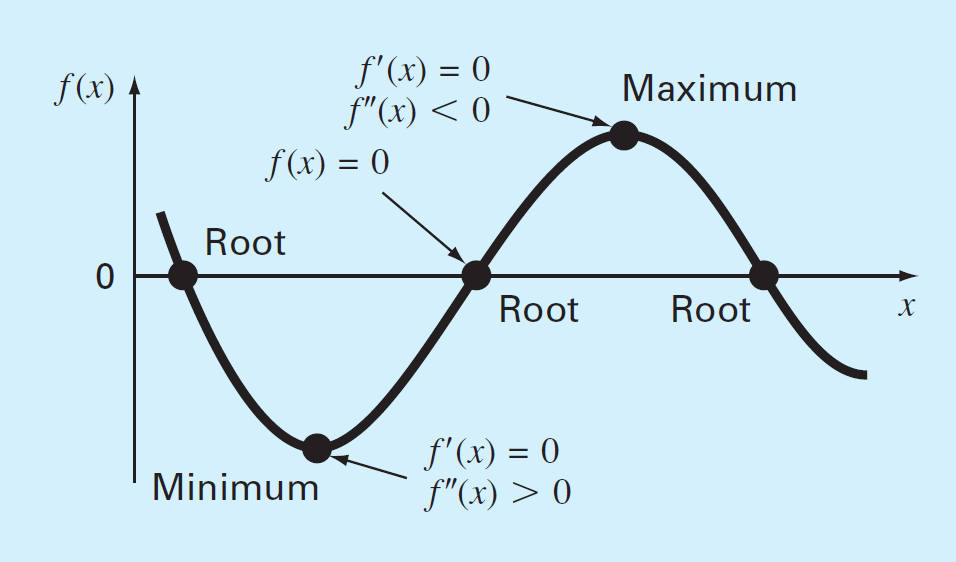
\includegraphics[width=0.6\linewidth]{./images/fig_pt_2_1}
    \caption{A function of a single variable illustrating the difference between roots and optima.}
\end{figure}

Such haphazard methods are obviously inefficient and inadequate for the requirements
of engineering and science practice. Numerical methods represent alternatives that are also
approximate but employ systematic strategies to home in on the true root. As elaborated in
the following pages, the combination of these systematic methods and computers makes
the solution of most applied roots-of-equations problems a simple and efficient task.\\

Besides roots, another feature of interest to engineers and scientists are a function's
minimum and maximum values. The determination of such optimal values is referred to as
\emph{optimization}. As you learned in calculus, such solutions can be obtained analytically by determining
the value at which the function is flat; that is, where its derivative is zero. Although
such analytical solutions are sometimes feasible, most practical optimization problems require
numerical, computer solutions. From a numerical standpoint, such optimization methods are
similar in spirit to the root-location methods we just discussed. That is, both involve guessing
and searching for a location on a function. The fundamental difference between the two types
of problems is illustrated in Figure PT2.1. Root location involves searching for the location
where the function equals zero. In contrast, optimization involves searching for the function's
extreme points.\\
\bigskip

\section[PART ORGANIZATION]{PART ORGANIZATION}

\noindent
The first two chapters in this part are devoted to root location. \emph{Chapter 5} focuses on \emph{bracketing methods} 
for finding roots. These methods start with guesses that bracket, or contain,
the root and then systematically reduce the width of the bracket. Two specific methods are
covered: \emph{bisection} and \emph{false position}. Graphical methods are used to provide visual insight
into the techniques. Error formulations are developed to help you determine how much
computational effort is required to estimate the root to a prespecified level of precision.

\emph{Chapter 6 covers open methods}. These methods also involve systematic trial-and-error
iterations but do not require that the initial guesses bracket the root. We will discover that
these methods are usually more computationally efficient than bracketing methods but that
they do not always work. We illustrate several open methods including the \emph{fixed-point
iteration, Newton-Raphson}, and \emph{secant} methods.

Following the description of these individual open methods, we then discuss a hybrid
approach called \emph{Brent's root-finding} method that exhibits the reliability of the bracketing
methods while exploiting the speed of the open methods. As such, it forms the basis for
MATLAB's root-finding function, \texttt{fzero}. After illustrating how \texttt{fzero} can be used for engineering
and scientific problems solving, Chap. 6 ends with a brief discussion of special
methods devoted to finding the roots of \emph{polynomials}. In particular, we describe MATLAB's
excellent built-in capabilities for this task.

Chapter 7 deals with \emph{optimization}. First, we describe two bracketing methods, \emph{goldensection
search} and \emph{parabolic interpolation}, for finding the optima of a function of a single
variable. Then, we discuss a robust, hybrid approach that combines golden-section search
and quadratic interpolation. This approach, which again is attributed to Brent, forms the
basis for MATLAB's one-dimensional root-finding function: \texttt{fminbnd}. After describing
and illustrating \texttt{fminbnd}, the last part of the chapter provides a brief description of optimization
of multidimensional functions. The emphasis is on describing and illustrating the
use of MATLAB's capability in this area: the \texttt{fminsearch} function. Finally, the chapter
ends with an example of how MATLAB can be employed to solve optimization problems
in engineering and science.

\end{document}